\documentclass{article}
\usepackage{pgf,tikz,tikzscale} 
\usepackage{amssymb}
\usepackage{tcolorbox}
\usepackage{xcolor}
\usepackage[utf8]{inputenc}
\usepackage[english]{babel}
\usepackage{multicol}
\usepackage{enumerate}	
\usepackage{graphicx,lipsum,pgfplots} 
\usepackage{amsmath, amsthm}                 
\usepackage[top=1in,bottom=1in, left=1in, right=1in] {geometry}  
\usepackage{fancyhdr}       
\usepackage{blkarray}


\pagestyle{fancy}              
\lhead{Math 5563 \newline Graph Theory HW4, Ch3}   
\rhead{Warren Keil}







\begin{document}
\setlength{\parindent}{0cm}   %%%%%%%% KEEP THIS  for block style paragraphs. 



\textbf{2.} Determine the connectivity \(\kappa(G)\) of the graphs in Exercise 1. 
\begin{center}
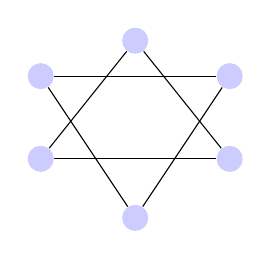
\begin{tikzpicture}
  [scale=.15,auto=left,every node/.style={circle,fill=blue!20}]
  \node (a) at (0,0) {};
  \node (c) at (-8,12)  {};
  \node (b) at (-8,5)  {};
  \node (e) at (0,15)  {};
  \node (f) at (8,12)  {};
   \node (g) at (8,5)  {};


  \foreach \from/\to in {a/c,a/f,c/f, b/e,b/g,e/g}
    \draw (\from) -- (\to);

\end{tikzpicture}\hspace{6mm}
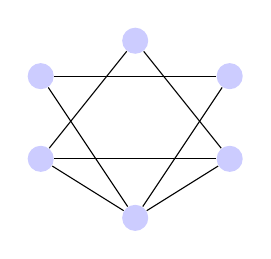
\begin{tikzpicture}
  [scale=.15,auto=left,every node/.style={circle,fill=blue!20}]
  \node (a) at (0,0) {};
  \node (c) at (-8,12)  {};
  \node (b) at (-8,5)  {};
  \node (e) at (0,15)  {};
  \node (f) at (8,12)  {};
   \node (g) at (8,5)  {};


  \foreach \from/\to in {a/c,a/f,c/f, b/e,b/g,e/g, a/b,a/g}
    \draw (\from) -- (\to);

\end{tikzpicture}\hspace{6mm}
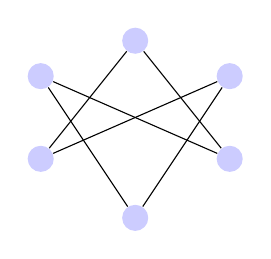
\begin{tikzpicture}
  [scale=.15,auto=left,every node/.style={circle,fill=blue!20}]
  \node (a) at (0,0) {};
  \node (c) at (-8,12)  {};
  \node (b) at (-8,5)  {};
  \node (e) at (0,15)  {};
  \node (f) at (8,12)  {};
   \node (g) at (8,5)  {};


  \foreach \from/\to in {a/c,a/f,e/b,e/g,c/g,f/b}
    \draw (\from) -- (\to);

\end{tikzpicture}  \hspace{6mm}
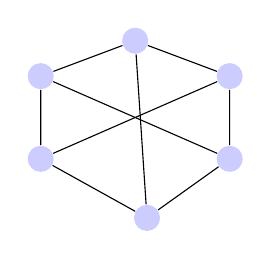
\begin{tikzpicture}
  [scale=.15,auto=left,every node/.style={circle,fill=blue!20}]
  \node (a) at (1,0) {};
  \node (c) at (-8,12)  {};
  \node (b) at (-8,5)  {};
  \node (e) at (0,15)  {};
  \node (f) at (8,12)  {};
   \node (g) at (8,5)  {};


  \foreach \from/\to in {a/b,b/c,c/e,e/f,f/g,a/g, a/e, b/f,c/g}
    \draw (\from) -- (\to);

\end{tikzpicture}
\end{center}

\textit{Solution} Let \(G_i\) for \(i \in \{1,2,3,4\} \) be the graphs in order as illustrated above. We see that \(\kappa(G_1)=0\) since \(G_1\) already has two components. Next, we see that \(\kappa(G_2)=1\) since \(G_2\) becomes disconnected by removing the bottom vertex. Next, we observe that \(G_3\) is really just \(C_6\), and so \(\kappa(G_3)=\kappa(C_6)=2\). And lastly, we show by exhausting all cases that \(\kappa  G_4=3\). We first remove one vertex and see that \(G_4\) is connected. Notice it does not matter which vertex we remove since this graph is symmetric. Next, we check the result of removing each additional vertex and find that the graph is still connected. So \(\kappa(G_4) >2\). But observe that if we remove every other vertex of \(G_4\) we are left with a disconnected set. Thus \(\kappa(G_4)=3\). 



\vspace{5mm}

\textbf{4.} Find the flaw in the following proof: If \(\varepsilon(G)=0\), then \(G=K_1\) or \(G\) is disconnected, in which cases \(\kappa(G) = \varepsilon(G)\). Otherwise, suppose \(\varepsilon(G)=t>1\) and let \(\{e_1,e_2,\ldots,e_t\}\) be a disconnecting set of edges of \(G\). If \(e_i=\{u_i,v_i\},1\leq i \leq t\), then \(S=\{u_i :1\leq i\leq t\}\) is a vertex cut. Hence, \(\varepsilon(G) = t \geq o(S) \geq \kappa(G)\).

\vspace{3mm}

\textit{Solution.} The first minor error in this proof is that it does not cover the case when \(\varepsilon(G)=1\). It states that fact about the case when \(\varepsilon(G) = 0\) and then moves on to the cases when \(\varepsilon(G)>1\). The main flaw of this proof is the statement, \textit{If \(e_i=\{u_i,v_i\},1\leq i \leq t\) is a disconnecting set, then \(S=\{u_i :1\leq i\leq t\}\) is a vertex cut}. To see why this statement is false, consider \(K_5\). Let \(e_i=\{u_i,v_i\},1\leq i \leq 4\) be the smallest disconnecting set of edges, \(\varepsilon(G)\). Since our graph is \(K_5\), then it is trivially shown that the smallest disconnecting set consists of all the edges required to isolate a single vertex.  Then the set \(S\) as defined as \(S=\{u_i :1\leq i\leq t\}\) either contains one vertex or four. In either case the graph \(G-S\) is still connected as illustrated below. Another way to state this is that \(G-S\) either becomes the middle graph or the single vertex on the right of the graphs below. 
\begin{center}
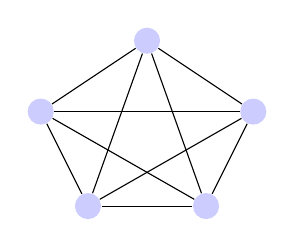
\begin{tikzpicture}
  [scale=.15,auto=left,every node/.style={circle,fill=blue!20}]
  \node (a) at (5,14)  {};
  \node (b) at (14,8)  {};
  \node (c) at (10,0)  {};
  \node (d) at (0,0)  {};
  \node (e) at (-4,8)  {};

  \foreach \from/\to in {a/b,a/c,a/d,a/e,b/c,b/d,b/e,c/d,c/e,d/e}
    \draw (\from) -- (\to);

\end{tikzpicture}\hspace{9mm}
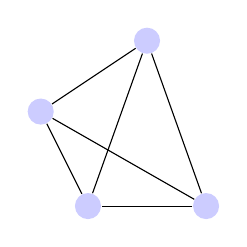
\begin{tikzpicture}
  [scale=.15,auto=left,every node/.style={circle,fill=blue!20}]
  \node (a) at (5,14)  {};
  %\node (b) at (14,8)  {};
  \node (c) at (10,0)  {};
  \node (d) at (0,0)  {};
  \node (e) at (-4,8)  {};

  \foreach \from/\to in {a/c,a/d,a/e,c/d,c/e,d/e}
    \draw (\from) -- (\to);

\end{tikzpicture}\hspace{9mm}

\begin{tikzpicture}
  [scale=.15,auto=left,every node/.style={circle,fill=blue!20}]
  \node (b) at (14,14)  {};

  \foreach \from/\to in {}
    \draw (\from) -- (\to);

\end{tikzpicture}\hspace{6mm}
 \end{center}
In either case, since we have shown that \(G-S\) is connected, then \(S\) is not a vertex cut.
\begin{flushright}
 \(\qed\) 
\end{flushright}





\newpage
\textbf{5. Corollary 3.4} \textit{ Suppose G is a connected graph. Let e = uv \( \in E(G)\). Then e is a bridge if and only if no cycle of G contains contains both u and v}.
\vspace{2mm}

\textit{Proof.} Let \(G=(V,E)\) be a connected graph. Let \(e = uv \in E(G) \). First, suppose that \(e\) is a bridge. Then by theorem 3.3, we know that the only path from \(u\) to \(v\) is \(P=[u,v]\). Then this clearly cannot be a cycle since it is a path of length 1. And furthermore, the theorem shows that this must be the only path from \(u\) to \(v\) which means these vertices cannot possibly be in another path and thus a cycle. 

Next, we show the opposite direction by the contrapositive. So assume that \(e\) is not a bridge and note that the term bridge is synonymous with cut-edge. Then by theorem 3.3, we know that the path \(P=[u,v]\) is not the only path from \(u\) to \(v\). Thus, there exist another path, call it \(P'\), such that \(P' = [ u, x_1, x_2, \dots, x_k, v] \) for some \( k \in \mathbb{N}\). We know that \(k\geq1\) since if \(k=0\), then \(G\) would no longer be a simple graph. So since these two distinct paths exist, and they both have endpoints of \(u\) and \(v\), then we can construct a cycle by starting with \(P'\) and then attaching the path \(P\) to connect \(u\) and \(v\). Thus we have shown there must exist a cycle that connects \(u\) to \(v\). Hence, if \(e\) is not a bridge, then there always exists a cycle of \(G\) that connects \(u\) to \(v\). Therefore, if no cycle of \(G\) contains both \(u\) and \(v\), then \(e\) must be a bridge. 

\begin{flushright}
 \(\qed\) 
\end{flushright}



\vspace{4mm}


\vspace{4mm}

\textbf{7 a.} Prove that \(\kappa(G)\) is invariant. 

\vspace{2mm}

\textit{Proof.} Let \(G=(V_1, E_1) \) and \(H=(V_2,E_2)\) be simple graphs such that \(G \cong H\). Let \(f:V_1 \rightarrow V_2\) be the corresponding isomorphism. Suppose \(\kappa(G)=k\). Then there exists a separating set \(S= \{v_1,v_2, \ldots, v_k\} \subseteq V_1 \) such that \( |S| = k \) and \(G-S\) is disconnected. And since this is the smallest separating set, then any other separating set will have at least as many elements as \(S\). Next, partition \(V_1\) into the two components we are guaranteed to have with \(G-S\). Name these two components of \(G-S\), \(\hat V_1\) and \(\bar V_1\). Next, let \(S' = f[S] = [f(v_1), f(v_2), \ldots, f(v_k)]\), let \( \hat V_2 = \{ f(v) : v \in \hat V_1\} \)  and let \( \bar V_2 = \{ f(v) : v \in \bar V_1\} \).  To show that \(S'\) is a separating set by contradiction, let \(v_2 \in \hat V_2 \) and \(u_2 \in \bar V_2\), and suppose there is some path in \(H-S\) from \(v_2 \) to \(u_2\). Then this path consists of vertices with that property that it starts at \( v_2 \in \hat V_2 \) and end with the vertex \(u_2 \in \bar V_2\). Then there must exist a path in \(G-S\) that starts at \( f^{-1}(v_2) \in \hat V_1\) and ends at \(f^{-1}(u_2) \in \bar V_2 \). But this cannot happen since \((G-S)[\hat V_1] \) and \( (G-S)[\bar V_1]\) are different components of \( (G-S)\). \( \rightarrow\!\leftarrow\) Thus, \(H-S'\) must be disconnected. Thus, \(S'\) must be a separating set. To show that \(S'\) is the smallest separating set by contradiction, suppose there is a smaller separating set of \(H\) called \(S''\) such that \( |S''| <|S'|\). Then using the same argument we used to show that \(S'\) is a separating set with \(k\) elements,  there must exist another separating set in \(G\) with the same number of elements as \(S''\). But this breaks are statement that the smallest separating set of \(G\) was of order \(k\). \( \rightarrow\!\leftarrow\) Therefore \(S'\) is the smallest separating set of \(H\). \(\therefore \kappa(H)=k\). \(\therefore \kappa(G)\) is invariant.
\begin{flushright}
 \(\qed\) 
\end{flushright}


\vspace{2mm}

\textbf{7b.} Prove that \(\varepsilon(G)\) is invariant. 

\vspace{3mm}

\textit{Proof.} Let \(G=(V_1, E_1) \) and \(H=(V_2,E_2)\) be simple graphs such that \(G \cong H\). Let \(f:V_1 \rightarrow V_2\) be the isomorphism. Let the edge connectivity of \(G\), \( \varepsilon(G) = k \). The the smallest disconnecting set of edges \(D\) has order \(k \). Partition \(V_1\) into the two components we are guaranteed to have with \(G-D\). Name these two components of \(G-D\), \(\hat V_1\) and \(\bar V_1\). Let \( \hat V_2 = \{ f(v) : v \in \hat V_1\} \)  and let \( \bar V_2 = \{ f(v) : v \in \bar V_1\} \). Let \(D' = \{ f(u)f(v) : uv \in D \} \). Then we will show that \(D'\) is a smallest disconnecting set in \(H\) and \(\hat V_2 \) and \(\bar V_2\) are the two disconnected components. To first show that \(H-D\) is disconnected, suppose there exist a past from some vertex in \(\hat V_2\) to \(\bar V_2\). Then since \(f\) is a bijection, there must also exist corresponding path from \(\hat V_1\) to \(\bar V_1\)  \( \rightarrow\!\leftarrow\). This surely cannot happen since \(\hat V_1\) and \(\bar V_1\) are disconnected. To show that \(D'\) is a smallest disconnecting set, suppose there is a smaller disconnecting set, \(D''\). Then by the same argument we used to show that \(D' =  \{ f(u)f(v) : uv \in D \} \) is a disconnecting set in \(H\), there must exist another disconnecting set \( D''' = \{ f^{-1}(u)f^{-1}(v) : uv \in D'' \} \). But this set must have the same number of edges as \( D''\) which is less then D  \( \rightarrow\!\leftarrow\). This surely cannot happen since \(D\) is the smallest disconnecting set. Thus, \(D'\) must be a smallest disconnecting set in \(H\). \(\therefore \varepsilon(G)\) is invariant. \begin{flushright} \(\qed\) \end{flushright}
\newpage
\textbf{24 a.} Find the girth of the graph in Figure 3.12. 
\vspace{3mm}

\textit{Solution.} By inspection, we see that the girth of this graph is three. 

\vspace{4mm}

\textbf{24 b.} Find the curcumference of the graph in Figure 3.12. 
\vspace{3mm}

\textit{Solution.} By inspection, we see that the circumference of this graph is seven. We know it is seven because there is an easy path to see that goes around the outside of the graph. And it uses every vertex. So there cannot be a longer path since a path cannot be longer than the number of vertices. 

\vspace{4mm}

\textbf{24 c.} Prove that \(g\leq 2d+1\), where \(d=\text{diam} (G) \) is the diameter of \(G\).  
\vspace{3mm}

\textit{Proof.} Let \(G\) be a two-connected graph with girth \(g\), and circumference \(c\). First observe that for any cycle with \(n\) vertices or edges, the maximum distance between any two vertices is \(\lfloor \frac n2 \rfloor\). Suppose that \( g>2d+1\). Then \(g \) has more than \(2d+1\) vertices. Then it follows that the diameter of \(g\) is 

\begin{align*}
 \text{diam}(g) &> \lfloor \frac{2d+1}{2} \rfloor \\
 &> \lfloor d + \frac12 \rfloor \\
 &> d\\
 &   \rightarrow\!\leftarrow
\end{align*}
This surely cannot be true since \(d\) is the maximum distance in \(G\). \(\therefore g\leq 2d+1\).
\begin{flushright}
 \(\qed\) 
\end{flushright}

\vspace{4mm}


\textbf{24 d.} Prove or disprove that any two cycles of \(G\) of length \(c\) must have at least two vertices in common if \(G\) is two connected. 
\vspace{3mm}

\textit{Proof.} Let \(G\) be a two connected graph with circumference \(c\). Let \(C_1, C_2\) be two cycles in \(G\) such that they both have length \(c\). To show that they must share at least two vertices in common, we will show by contradiction that they cannot share zero or only one vertex. 

\vspace{2mm}
\textit{Case 1:}  \(C_1\) and \(C_2\) share zero vertices. Then since \(G\) is a simple graph and two connected, then there must exist at least two distinct paths from \(C_1\) to \(C_2\) ( or else we could easily show that \(G\) is not 2-connected) Let \(C'\) be the cycle constructed by these two paths from \(C_1\) to \(C_1\) as well as the longest distance around each of \(C_1\) and \(C_2\) to the other path. Then if \(n\) is the number of vertices in \(c\), then it follows that 

\begin{align*}
C' &\geq 2 + 2( c - \lfloor \frac{n}2 \rfloor ) \\
&\geq  2 + 2c-n\\
&\geq 2 +c \\
&> c
\end{align*}
But this cannot happen since \(c\) is the longest cycle of \(G\). \( \rightarrow\!\leftarrow\)

\newpage
\textit{Case 2:}  \(C_1\) and \(C_2\) share one vertex. Since \(G\) is two-connected, then there must exist another path from \(C_1\) to \(C_2\). The shortest this path can be is length one. Let \(C'\) be the maximum cycle that consist of the two cycles \(C_1\) and \(C_2\) but also connecting at this new path of at least length one. Then if \(n\) is the number of vertices in \(c\), we have 

\begin{align*}
C' &\geq 1 + 2( c - \lfloor \frac{n}2 \rfloor ) \\
&\geq  1 + 2c-n\\
&\geq 1 +c \\
&> c
\end{align*}
Again, we know this cannot happen since \(c\) is the longest cycle of \(G\). \( \rightarrow\!\leftarrow\) So we have shown that the number of vertices shared by \(C_1\) and \(C_2\) cannot be equal to zero or one. Therefore, any two cycles of length \(c\) a 2-connected simple graph must share two or more vertices. 
\begin{flushright}
 \(\qed\) 
\end{flushright}






\vspace{4mm}
\textbf{25.} Find \(\kappa(G), \psi_G(u,v)\) and \(\psi_G(u,w)\). 

\vspace{3mm}
\textit{Solution.} By inspection, we see that \(\kappa(G) = 2\). \(\psi_G(u,v) = 3\). \(\psi_G(u,w)=2\). 

















\end{document}
